\begin{quote}
{\em Before EDA, integrated circuits were designed by hand.} -- Daniel Nenni~\cite{wikicite}
\vspace{-2mm}
\end{quote}

\section{Introduction}

The Internet has been an amazing success for nearly 50 years, partly because of a key design decision to make the network “application agnostic”.   In other words, IP treats all applications – whether remote tele-surgery or Facebook – as a group of addresses that send a bag of bits to each other.  
This allowed the Internet to start with apps like email, and later accommodate unforeseen applications like video. Today we take for granted services like Uber for hailing a cab but these run on cheap computers connected by an IP data center network.  There many more exciting networked applications around the corner whether networks of self-driving cars, remote telesurgery, precision agriculture, and more we don’t know of.

Many of these new applications are critical.  They are so essential for society that they demand unprecedented levels of performance and reliability from the network.  For example, a storage area network may require the network to deliver a disk block in $<$ 100 usec, and cloud services aspire to 5 9s reliability.  The requirements for networks of self-driving cars, for augmented reality, and for remote tele-surgery are still being formulated.

While such stringent requirements are typically associated with large enterprises such as Google and Facebook with deep pockets and armies of experts, what is surprising is how such requirements also flow to lower tier networks where expertise is scarce and cost is an issue.  Consider for example, a surgeon doing remote telsurgery from Tamil Nadu to a village 100 miles away.  Such a network has tremendous requirements on latency and jitter, and customizing such a network could help save costs or even lives.

Networks today are managed using a patchwork of complex, manual, and low-level mechanisms. Network architects produce designs largely by hand, guided by intuition and experience. Network operators reconfigure network devices constantly to match evolving needs, leading to configurations that are inefficient, difficult to understand, and ever more brittle. 

As a result, networks today suffer from {\em high cost} (Google~\cite{b4} reports a factor of two underutilization for expensive transoceanic links), {\em high latency} (Amazon~\cite{amazon} asserts that a 100ms increase in latency leads to a 1\% drop in revenue), {\em lack of agility} (a startup~\cite{mahajan} reports that some Fortune 500 companies take over a week to roll out minor configuration changes because they do not fully understand their potential impact), {\em fragility} (surveys~\cite{atpg} have shown that one in three networks have dozens of incidents per month that take over an hour to resolve), {\em insecurity} (denial-of-service attacks now account for 16\% of network attacks~\cite{calyptix}), and {\em high barriers to entry} (rural networks cannot afford to employ hundreds of highly-trained operators~\cite{barathwisp}).

Companies such as Microsoft that traditionally distributed software on disks have transitioned to a cloud-hosted service model through products such as Office365. Gartner estimates the size of the current public and private cloud markets at \$139B and \$10B respectively. The poor performance and fragility of networks has direct negative impacts on cloud computing. For example, Google aims to limit downtime to ``a few minutes per month''~\cite{rameshgoogle}---anything more would hurt their bottom line as they make only a few cents on each search query. 

In other fields, increasing scale and requirements led to intellectual advances in \emph{design automation}. For example, challenges related to scaling hardware designs in the 1970s led to the creation of electronic design automation (EDA) as an academic discipline~\cite{alberto} as well an entire industry of EDA tools (e.g., high-level synthesis, functional verification). Similarly, increasingly stringent requirements on large-scale software led to the theory and practice of high-level languages and companion technologies (compilers, integrated development environments).   McKeown~\cite{mckeown} suggests there is a large opportunity for automation, noting that in both software and chip worlds a \$10B tool industry supports a \$100B software and chip industry, but that networks largely lack such tools. 


\begin{quote}
{\em The earliest EDA tools were produced academically.} -- EDA
History~\cite{wikicite2}.
\vspace{-2mm}
\end{quote}


\paragraph*{Our Vision.}
%
Our central vision is to empower any enterprise – whether small or large, whether
a rural network in Mendocino County or a large data center in  Oregon -- to build and operate a customized network that provides the properties their application requires, while minimizing the number of manual effort required by network architects and  operators.

To do so, we are inspired by the transformative effects of software tools and EDA, a field of {\em Network Design Automation} (NDA). We plan to develop novel science and practical tools that will  revolutionize how networks are designed, managed, and evolved, thereby increasing the pace of innovation, reducing the cost of building secure, reliable, and performant services, and even lowering the barrier to entry for operators of rural networks and data centers, and possibly in the futiure
ISPs and cellular networks.

{\bf Why Now?} We believe the time is right for NDA, as evidenced by recent progress in academia and industry. In 2013, Google~\cite{b4} and Microsoft~\cite{swan} deployed new traffic engineering systems that compute efficient routes through the network automatically and without human intervention. They found that programming the network {\em as a whole} increased utilization and reduced cost by millions of dollars. We have built verification~\cite{veriflow,hsa,lam}, testing~\cite{atpg,nice}, and debugging~\cite{xtrace} tools, along with many others, and we have also designed higher-level languages for expressing network policies~\cite{netcore-popl12,netkat}. The number of papers on top-down design and verification at SIGCOMM, the flagship networking conference, grew from 1/30 before 2011 to 8/40 in 2016. Veriflow~\cite{veriflow} and Forward Networks~\cite{forward} received millions in venture capital funds in 2015 to verify network properties. In 2015, Cisco founded a design automation unit called Candid under Sundar Iyer~\cite{sundar}, and Amazon hired Byron Cook to create a cloud verification group~\cite{byron}.  While there has been a flurry of recent activity in 
design tools for clouds, initial work has also begun on network design for rural
networks~{barath}.

{\bf What's Left?} While these initial activities are promising, NDA will not happen without a significant, coherent, sustained effort that {\em democratizes} network design
and operation tools so that every network, from the smallest rural network to the
largest data center can systematically design and operate their networks to work at the highest levels of reliability and performance without a large team of operators that only the largest enterprises can afford.

In this context, the point solutions listed above are a great start, there are several gaps: {\em 1. Fundamental questions unanswered:}  For example, network reachability
approaches~\cite{hsa,veriflow} break down in the presence of stateful
devices such as firewalls.  More generally, there are no fundamental
models analogous to Turing machines, or general verification
abstractions akin to Hoare logic~\cite{Hoare69}. {\em 2. Most design
  is manual.} The design of a network, from its structure to its
components to its configuration, is largely done by hand. {\em
  3. Isolated abstractions:} Existing
abstractions~\cite{netkat,propane,hsa,Ethane,4DControlPlane} are promising but are neither
complete nor interconnected. {\em 4. Focus on data centers:} Most
extant work ignores diverse networks such
as rural networks. {\em  5. Few connections between
  interdisciplinary areas:} NDA encompasses a range of disciplines
spanning data mining to programming languages to ICDT and yet there have been
few attempts to bring researchers in different disciplines to work together
coherently. {\em 6. Limited outreach:} Existing tools (e.g., Batfish~\cite{batfish}, Propane~\cite{propane} are still not directly
applicable except to expert operators in larger networks.
The goal of this NSF Large is to fill these gaps with a significant, coherent, and
sustained effort in three areas:


% \begin{table}
% \begin{small}
% \centerline{
% \begin{tabular}{@{}|@{\,}c@{\,}|@{\,}c@{\,}|@{\,}c@{\,}|@{}}
% \hline
% {\bf Task} & {\bf Abstraction} & {\bf Sample Scientific Question} \\
% \hline High-Speed Packet Forwarding &
% Hardware tile description  &
% Can stochastic search help design hardware? \\
% \hline Flexible Router Compilers & IRs for Packet Processing & What is ``the LLVM'' for routers?\\
% \hline Topology Design & Topology Description Language & Can SAT Solvers aid topology design? \\
% \hline Network Management & Network Policy Language & How to apply stepwise refinement to networks? \\
% \hline Network Monitoring & Performance Query Language & How to map performance assertions to routers? \\
% \hline Failure Analysis & Cause-effect Graphs & Can NLP find causal relations from text? \\
% \hline
% \end{tabular}
% }
% \end{small}
% \caption{Sample tasks, abstractions, and scientific questions for our proposed research on NDA.}
% \label{scientificquestions}
% \end{table}

\begin{figure}[t]
\centerline{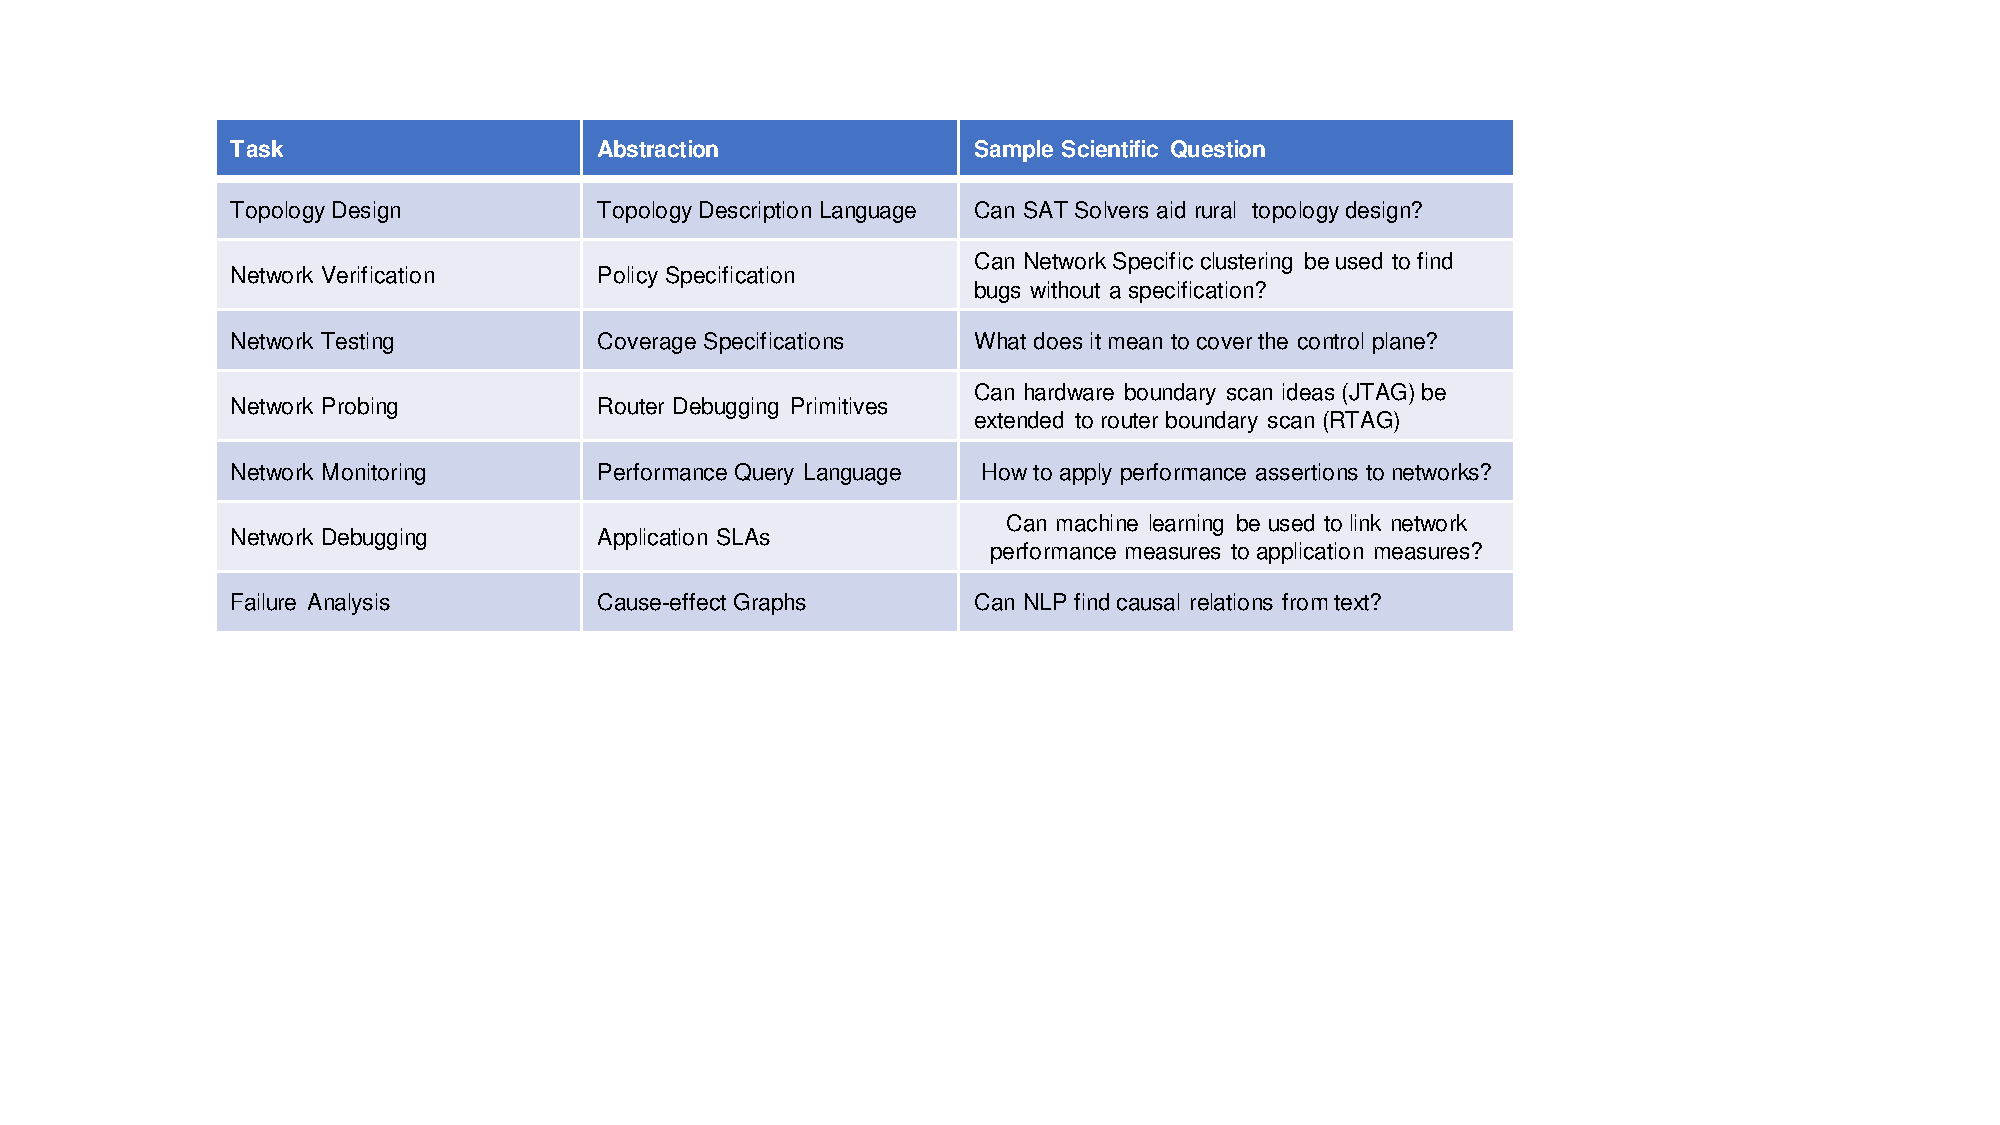
\epsfig{file=questions_table.pdf, height=5in}}
\caption{Sample tasks, abstractions, and scientific questions for our
  proposed research on NDA.}
\vspace{2mm}
\label{scientificquestions}
\end{figure}


\paragraph*{1. Intellectual Merit: NDA Science.} {\em We will develop a science of network design automation, inspired by programming methodologies but united by an emphasis on domain-specific languages and algorithmic search techniques.}
%
On the surface, networks with their collections of routers, interface cards, and links do not resemble software. But one can view the entire network as a ``program'' that takes packets at the incoming edge of the network and outputs packets at the outgoing edge, after possibly rewriting some of the bits in the packet. For instance, a forwarding table on an individual router can be viewed as a ``switch'' statement on the packet's destination addresses, while a link between routers can be viewed as an assignment statement that modifies the packet's location. These analogies suggest a new research agenda that asks: what languages and tools are needed to program and reason precisely about networks?  
However, solutions cannot merely reuse existing ideas from programming languages and related fields. Instead, effective solutions for network programming and verification will require new abstractions that tackle the unique challenges of the domain: networks are fundamentally asynchronous and distributed, the state space of possible packets is huge, and the correctness and performance requirements are subtle and complex. At the same time, networks have domain-specific structure that can be exploited by tools. For example, an off-the-shelf theorem prover for verifying network reachability took more than {\em 1 day}~\cite{nod} but by cleverly exploiting equivalences between configurations, Yang and Lam were able to complete the same task in under {\em 1 second}~\cite{lam}.
Table~\ref{scientificquestions} summarizes some of the language design and scientifc questions we will address and Figure~\ref{fig:pairwise} relates these questions to practical problems in various types of networks today.

\paragraph*{2. Broader Impact: Network Design Tools.}{\em We will build a suite of tools for networks to begin to catalyze an industry for Network Design Automation akin to the EDA industry.}   
%
 We imagine network architects at Fortune 500 companies and rural ISPs using NDA languages to develop designs in hours or days, lowering cost and increasing robustness. We expect network operators to be able to evolve a network in an agile fashion---e.g., reacting to traffic spikes, responding to security threats, and rolling out new services. While we do not propose to deliver industrial-strength tools, we plan to collaborate with established companies (VMWare, Cisco, Google, and Microsoft) and startups (Candid and Forward Networks) via internships and joint projects (see letters  attached to this proposal). We seek to develop the foundation of the NDA industry just as academia did for the EDA industry in the 1970s~\cite{alberto}.

\paragraph*{3. Broader Impact: NDA Education.} {\em We will take first steps toward lowering the educational barriers for people around the world to operate networks.}
%
As with the EDA and software revolutions, achieving wide impact will require educational materials to train the next generation to use NDA methodologies and technologies. To enfranchise operators, we will focus on producing open-source course material (inspired by Khan Academy) based on what we call {\em network scripting} that will teach how to manage the vast majority of simple networks found around the world, together with open-source simulators for easy network testing. We seek to complement existing efforts such as Cisco Academy~\cite{ciscoacademy} that have already had major impact in disadvantaged societies. 

{\bf Why an NSF Large?}  While individual researchers and companies can build impressive point solutions (e.g., ~\cite{b4}), it takes the efforts of several researchers working in concert to map out the landscape of NDA and define its interconnections (see Figure~\ref{fig:abstractions}). Networking spans a range of disciplines including language design, verification, testing, debugging, and data mining. Our team brings together networking experts (Varghese, Govindan, both ACM Fellows for networking), with PL expert Millstein (who helped found the nascent field of network verification) and domain experts in ICTD (Raghavan), debugging (Netravali), and systems testing (Tamir) to facilitate interdisciplinary exploration at a much larger scale than is possible in a smaller NSF grant.  

All six researchers, however, are in Los Angeles at UCLA and USC. Further, many of them have worked together successfully in research teams (e.g., Govindan-Varghese, Govindan-Millstein, Raghavan-Varghese) over many years and many projects. We believe colocation in Los Angeles facilitates genuine collaboration and frequent in-person meetings with students and PIs, in contrast to the more sprawling and comparitively isolated efforts of other multi-institution proposals.

{\bf Why not Industry?} Companies, which generally operate on short-term schedules dictated by the lifecycles of their products, are not incentived to organize a large-scale effort such as NDA, let alone tackle difficult scientific questions. Instead, we are inspired by Berkeley's early development of open-source products (e.g., the VLSI Tarball~\cite{wikicite}) and leadership (e.g., by Sangiovanni-Vincentelli and Newton) for EDA.  We note that three of us (Govindan, Millstein, Varghese) have been working to help pioneer this area for the last five years; we feel it is time to take the next step to consolidate this field further

\paragraph*{Related Efforts and Scope.}
%
First, the recent architectural shift known as software-defined networking (SDN) provides a set of basic mechanisms that allow network routers to be centrally programmed.  However, new mechanisms alone are not sufficient: we contend that NDA is necessary to fulfill the promise of SDN, just as higher-level languages and tools were necessary to fulfill the promise of VLSI. Further, NDA does not depend on SDN. Our focus is on building tools for existing networks in the next 5 years while laying a scientific foundation for the next 10 years of networking research. Second, while NDA encompasses aspects of security that are directly impacted by network design and operations, such as ensuring isolation and detecting attacks, other aspects of security, such as encryption and authentication, are out of scope for this project. Existing efforts at  UCLA~\cite{amitcenter} are already investigating these problems.  

Third, we will focus in this grant on verification and automation of the
design and operation of existing networks as opposed to more clean slate
approaches being pursued by our colleagues at Cornell (Foster) and Princeton (Rexford, Walker).  We fully intend to work with these colleagues wherever feasible, and will look for middle ground between their top-down language guided approaches.  For instance, Millstein and Varghese have an NSF Medium working
with Walker at Princeton on making the Propane language for router configurations more deployable.

Fourth, some of us (i.e., Varghese, Tamir) have expertise and interest in router
hardware design and emerging languages for reconfingurable routers like P4~\cite{P4} and believe that Network Design Automation in its most general form also applies to building tools like router compilers.  However, since tools for router design are cleanly separable from tools for network design, we will focus in this grant on
network tools {\em except} for router hardware debugging primitives to
assist network debugging.
